\documentclass[11pt]{article}

\usepackage{amsmath}
\usepackage{amssymb}
\usepackage{graphicx}
\usepackage[margin=1in]{geometry}
\usepackage{tikz}
\usetikzlibrary{arrows.meta, positioning, calc}
\usepackage{array}
\usepackage{booktabs}
\usepackage[table]{xcolor}

% Raggedright paragraph column type for tables (prevents ugly hyphenation)
\newcolumntype{R}[1]{>{\raggedright\arraybackslash}p{#1}}
\usepackage{hyperref}
\usepackage[numbers]{natbib}
\usepackage{fontspec}

% Avenir Ultra Light for figures and tables
\newfontfamily\avenirultralight{Avenir Next Ultra Light}

% Table styling: Avenir Ultra Light with alternating row shading
\definecolor{tableShade}{gray}{0.93}
\newcommand{\tablestyle}{\avenirultralight\small\renewcommand{\arraystretch}{1.35}}

% Use \avenirultralight in all TikZ node font= specifications
% Use \tablestyle in all table environments

\title{Decision-Valued Maps: A Diagnostic Infrastructure\\for Representational Dependence}
\author{Gil Raitses}
\date{}

\begin{document}

\maketitle

\begin{abstract}
Complex analytical pipelines produce discrete outcomes whose dependence on representational choices is rarely recorded or tested. A decision-valued map records which discrete outcome a fixed engine produces under each member of a declared family of representations, making that dependence an observable, storable object. This paper formalizes the concept and describes DecisionDB, a minimal infrastructure for logging, replaying, auditing such maps using content-addressed identifiers, immutable artifacts, declared equivalence policies. In a concrete decision setting on a fixed graph snapshot, two representation parameters are swept under a fixed computational engine. Sweeping the neighbor weight leaves decision identity unchanged across the tested range, while sweeping the second-order weight produces a boundary where the engine returns a distinct output path under identical query conditions. Deterministic replay recovers each decision identifier from its stored artifacts, establishing that the recorded context fully specifies the outcome. The contribution is infrastructural, establishing a system-level abstraction that partitions representation space into persistence regions and boundaries and treats decision reuse as a mechanically checkable condition.
\end{abstract}


\section{Introduction}

Analytical pipelines produce discrete outcomes that depend on how their inputs are represented. The same data, processed through the same computational engine under the same query, can yield different outcomes when the internal representation changes. Some representational changes leave the outcome intact; others alter it entirely.

This dependence arises from encoding choices such as which features are weighted, which aggregation rules are applied, which kernels are selected, because the outcome varies under representational change even when the engine and snapshot remain invariant. In current practice, a pipeline runs under one representation, a result is reported, the sensitivity of that result to representational alternatives remains invisible.

A \emph{decision-valued map} records which representations preserve the outcome and which change it, associating each member of a representation family with the discrete result the engine produces. By materializing this map across controlled representational variation, persistence regions where the outcome holds steady and boundaries where it changes become directly observable.

DecisionDB implements this protocol by logging every stage of the evaluation chain as a content-addressed artifact. It logs snapshots, representations, engine runs and decision identities using identifiers computed from content and artifacts stored in write-once form. It supports representational sweeps through systematic variation of declared representation parameters, replay verification through deterministic recovery of decision identifiers from persisted artifacts and post-hoc audit of the full provenance chain.

A graph routing problem provides the empirical setting. Holding a graph snapshot and a shortest-path engine constant, two representation parameters that control edge-cost construction are swept. One parameter preserves decision identity across its tested range; the other induces a discrete identity change at a specific threshold. Replay verification recovers all persisted identifiers exactly.

The contribution is an infrastructure that produces a queryable, replayable record of how discrete outcomes depend on representational choice.


\section{Problem Scope}

We consider systems with the following structure:

\begin{enumerate}
\item A \textbf{snapshot} $s$: a frozen, immutable slice of external inputs over a declared time window. Any change to the world state produces a new snapshot.
\item A \textbf{representation} $r \in \mathcal{R}(s)$: a deterministic encoding of $s$, defined by explicit structural choices (kernels, thresholds, weighting rules, aggregation policies). Each representation is fully specified by a declared parameter set and generated by a versioned factory.
\item A \textbf{engine} $E$: a fixed computational procedure that consumes a representation and produces raw output. Engine configuration and version are held constant during analysis.
\item An \textbf{equivalence policy} $\pi$: a declared rule that reduces raw engine output to a discrete \textbf{decision identity} $d \in \mathcal{D}$. The policy defines when two raw outputs correspond to the same identity, independent of incidental numerical differences.
\end{enumerate}

The scope is diagnostic: we characterize when decision identity persists across representational variation and when it changes. We do not introduce training procedures, adaptive updates, gradient-based optimization, or online learning. Continuous outputs are in scope only when reduced to discrete identities via a declared policy.

This framing applies wherever discrete outcomes emerge from complex pipelines and representational choices may influence those outcomes. Examples include routing under alternative cost encodings, classification under alternative feature constructions, and resource allocation under alternative aggregation rules.


\section{The Decision-Valued Map}

The central object of study is a mapping
\[
f \colon \mathcal{R} \to \mathcal{D},
\]
where $\mathcal{R}$ denotes a family of representations over a fixed snapshot $s$ and $\mathcal{D}$ denotes a set of discrete decision identities. For each representation $r \in \mathcal{R}$, the engine $E$ produces raw output $E(r)$, and the equivalence policy $\pi$ extracts a decision identity $d = \pi(E(r))$.

Three structural features of this map are observable through controlled variation of $\mathcal{R}$. Persistence regions are connected subsets of $\mathcal{R}$ over which $f$ is constant; within a persistence region, representational variation preserves the outcome. Boundaries are loci in $\mathcal{R}$ where $f$ changes value, separating two persistence regions with different decision identities. Fractures are boundaries where a small change in representation parameters induces a discrete identity change, indicating high sensitivity of the outcome to the representation.

The purpose of DecisionDB is to \emph{materialize} $f$, evaluating it at declared points in $\mathcal{R}$, storing the results as immutable artifacts, then making the resulting map queryable, replayable, auditable. Figure~\ref{fig:pipeline} illustrates this protocol.

\definecolor{erdHeader}{HTML}{e1d5e7}
\definecolor{erdStroke}{HTML}{b5739d}
\definecolor{arenaFill}{HTML}{f3eff7}

\begin{figure}[t]
  \centering
  \begin{tikzpicture}[
    box/.style={draw=erdStroke, rounded corners=4pt, align=center, inner sep=5pt, minimum height=13mm, font=\figfont\footnotesize, fill=erdHeader},
    smallbox/.style={draw=erdStroke, rounded corners=3pt, align=center, inner sep=4pt, minimum height=10mm, font=\figfont\scriptsize, fill=erdHeader!40},
    idbox/.style={draw=erdStroke, rounded corners=3pt, align=center, inner sep=3pt, minimum height=8mm, font=\figfont\scriptsize},
    arrow/.style={-{Latex[length=2.5mm, width=2mm]}, thick, erdStroke},
    eqlbl/.style={font=\figfont\scriptsize, erdStroke},
    arenalbl/.style={font=\figfont\scriptsize, text=black!65}
  ]

  % Arena enclosure
  \draw[erdStroke!40, rounded corners=6pt, fill=arenaFill] (-0.8, 1.0) rectangle (4.6, -0.7);
  \node[arenalbl, anchor=north west] at (-0.6, 0.9) {arena (invariant)};

  % Arena components inside the enclosure
  \node[box, text width=20mm] (snap) at (0.6, 0.2) {Snapshot $s$};
  \node[box, text width=20mm] (eng) at (3.4, 0.2) {Engine $E$};

  % Representation family (parallel, outside arena, feeding into engine)
  \node[smallbox, text width=22mm] (r1) at (7.0, 1.6) {$r_1$};
  \node[smallbox, text width=22mm] (r2) at (7.0, 0.2) {$r_2$};
  \node[smallbox, text width=22mm] (r3) at (7.0, -1.2) {$r_3$};
  \node[arenalbl, anchor=south] at (7.0, 2.2) {representation family};

  % Arrows from arena engine to each representation evaluation
  \draw[arrow] (eng.east) -- ++(0.4,0) |- (r1.west);
  \draw[arrow] (eng.east) -- (r2.west);
  \draw[arrow] (eng.east) -- ++(0.4,0) |- (r3.west);

  % Decision identifiers (output) -- grouped by agreement
  \draw[blue!8, rounded corners=4pt, fill=blue!6] (9.5, 2.1) rectangle (11.0, -0.3);
  \node[idbox, fill=blue!12] (d1) at (10.2, 1.6) {$d_A$};
  \node[idbox, fill=blue!12] (d2) at (10.2, 0.2) {$d_A$};
  \node[idbox, fill=orange!18] (d3) at (10.2, -1.2) {$d_B$};

  \draw[arrow] (r1.east) -- (d1.west);
  \draw[arrow] (r2.east) -- (d2.west);
  \draw[arrow] (r3.east) -- (d3.west);

  \end{tikzpicture}
  \caption{Evaluation protocol for a decision-valued map. A single arena, consisting of a data snapshot and a computational engine, is reused across evaluation. Representations drawn from a declared family are varied within this arena and evaluated independently. Agreement of decision identifiers across representations indicates persistence of decision identity; a change in identifier indicates a boundary induced by representational variation alone.}
  \label{fig:pipeline}
\end{figure}


\section{Sweep Protocol}

A \emph{representational sweep} evaluates the decision-valued map $f$ across a declared set of representations. The protocol proceeds in five stages:

\begin{enumerate}
\item \textbf{Freeze snapshot.} A snapshot $s$ is frozen and assigned a content-addressed identifier computed from its canonical JSON serialization (SHA-256, truncated to 16 hex characters, prefixed with \texttt{snap\_}).

\item \textbf{Declare representations.} A representation family $\mathcal{R}(s)$ is declared, along with a deterministic factory that generates individual representations from parameter settings. Each representation receives a content-addressed identifier (prefix \texttt{repr\_}). Representation parameters are explicitly separated from engine configuration.

\item \textbf{Plan sweep.} A sweep plan specifies the parameter grid to be evaluated, the engine name and version, and the equivalence policy. The plan itself is content-addressed.

\item \textbf{Execute engine.} The fixed engine is executed independently for each representation. Each run produces a raw output artifact stored as an immutable file, linked by content hash (prefix \texttt{run\_}). Engine configuration is held constant across the sweep.

\item \textbf{Extract decisions.} The equivalence policy $\pi$ is applied to each raw output to produce a discrete decision identity (prefix \texttt{dec\_}). The decision map table records the link from representation to engine run to decision identity.
\end{enumerate}

All artifacts are versioned and linked through content-addressed identifiers. The resulting materialized map supports reproducible replay and post-hoc analysis without re-executing the engine.


\section{System Design}

DecisionDB is implemented as a Python package backed by SQLite. It manages five entity types through a relational schema with content-addressed primary keys and foreign-key constraints.

\subsection{Content Addressing}

All identifiers are computed deterministically from content. Given an entity's payload as a Python dictionary, DecisionDB serializes it to canonical JSON with keys sorted alphabetically, no whitespace, arrays in declaration order, floats as strings, and explicit version fields. It then computes the SHA-256 digest of the UTF-8 encoding, truncates to the first 16 hexadecimal characters, and prepends a type-specific prefix. Identical content always produces identical identifiers, regardless of when or where the computation occurs.

\subsection{Schema}

The relational schema contains five core tables. Figure~\ref{fig:schema} shows their foreign-key relationships and Table~\ref{tab:schema} summarizes each table's role. Each table enforces content-addressed primary keys and foreign-key constraints that link the full provenance chain from snapshot through representation and engine execution to decision identity. All writes are append-only, scoped by experiment identifier, and executed within transactions. Inserts use an insert-or-ignore strategy for idempotency, so re-inserting the same content-addressed entity is a no-op.

\begin{figure}[t]
  \centering
  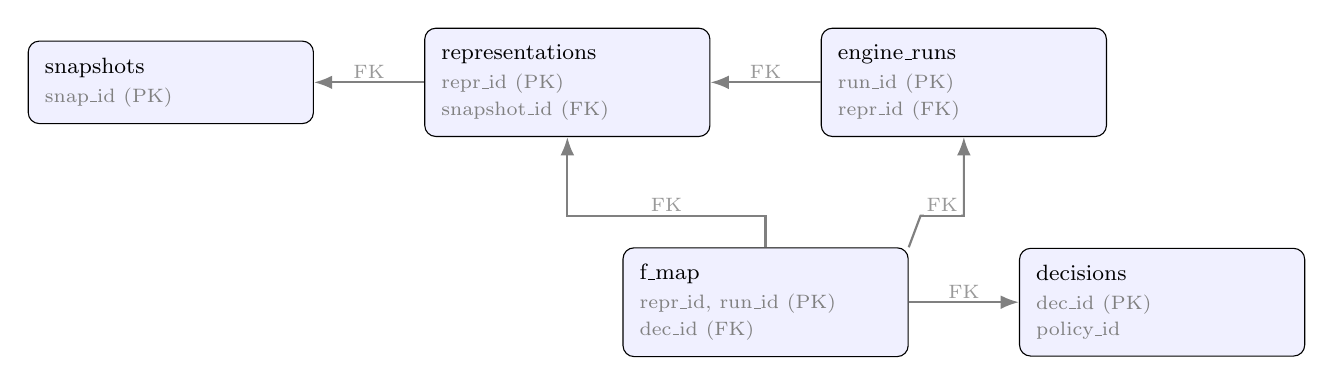
\begin{tikzpicture}[
    node distance=8mm and 14mm,
    entity/.style={draw, rounded corners, align=left, inner sep=6pt, text width=32mm, font=\avenirultralight\footnotesize, fill=blue!6},
    fk/.style={-Latex, thick, black!50},
    fklbl/.style={font=\avenirultralight\scriptsize, text=black!40, fill=white, inner sep=1pt}
  ]

  \node[entity] (snap) {%
    snapshots\\[1pt]
    {\scriptsize\color{black!50} snap{\_}id (PK)}};

  \node[entity, right=of snap] (repr) {%
    representations\\[1pt]
    {\scriptsize\color{black!50} repr{\_}id (PK)}\\
    {\scriptsize\color{black!50} snapshot{\_}id (FK)}};

  \node[entity, right=of repr] (runs) {%
    engine{\_}runs\\[1pt]
    {\scriptsize\color{black!50} run{\_}id (PK)}\\
    {\scriptsize\color{black!50} repr{\_}id (FK)}};

  \node[entity, below=14mm of $(repr.south)!0.5!(runs.south)$] (fmap) {%
    f{\_}map\\[1pt]
    {\scriptsize\color{black!50} repr{\_}id, run{\_}id (PK)}\\
    {\scriptsize\color{black!50} dec{\_}id (FK)}};

  \node[entity, right=of fmap] (dec) {%
    decisions\\[1pt]
    {\scriptsize\color{black!50} dec{\_}id (PK)}\\
    {\scriptsize\color{black!50} policy{\_}id}};

  \draw[fk] (repr.west) -- node[fklbl, above] {FK} (snap.east);
  \draw[fk] (runs.west) -- node[fklbl, above] {FK} (repr.east);
  \draw[fk] (fmap.north) -- ++(0,0.4) -| node[fklbl, near start, above] {FK} (repr.south);
  \draw[fk] (fmap.north east) -- ++(0.15,0.4) -| node[fklbl, near start, above] {FK} (runs.south);
  \draw[fk] (fmap.east) -- node[fklbl, above] {FK} (dec.west);

  \end{tikzpicture}
  \caption{DecisionDB relational schema. Five tables form a content-addressed provenance chain. Foreign-key arrows indicate the direction of referential dependency, linking representations to their parent snapshot, engine runs to the representation consumed, and the decision map table to representations, runs, and decision identities.}
  \label{fig:schema}
\end{figure}

\begin{table}[t]
\centering
\caption{DecisionDB entity roles.}
\label{tab:schema}
\smallskip
\tablestyle
\rowcolors{2}{tableShade}{white}
\begin{tabular}{@{\hskip 8pt}l l R{68mm}@{\hskip 8pt}}
\toprule
\rowcolor{white}
Table & Key prefix & Role \\
\midrule
snapshots & snap & Immutable frozen input state and its artifact manifest \\
representations & repr & Deterministic encodings of snapshots under a declared parameterization \\
engine runs & run & Execution records of the fixed engine on specific representations \\
decisions & dec & Discrete decision identities extracted by an equivalence policy \\
f map & composite & Materialized decision-valued map linking representations, runs, and decisions \\
\bottomrule
\end{tabular}
\end{table}

\subsection{Equivalence Policies}

An equivalence policy defines how raw engine output is reduced to a decision identity. Each policy specifies a hash source, identifying which field of the raw output carries decision-relevant content such as the route node sequence. It also specifies a canonicalization rule that determines how to serialize the extracted content, and a match rule that determines identity such as SHA-256 equality. The policy itself is content-addressed, so any change to the policy definition produces a new policy identifier and new decision identifiers downstream.

\subsection{Replay Verification}

Replay verification takes a persisted decision record, reloads the stored raw output and policy specification, recomputes the policy identifier, payload hash, and decision identifier, and checks them against the persisted values. Because replay is read-only and writes no rows, a successful pass confirms that the content-addressing chain from raw output through policy application to decision identity is deterministic and self-consistent.


\section{Empirical Demonstration}

We demonstrate the framework on a graph routing problem. The goal is not to evaluate routing algorithms, but to show how the decision-valued map makes representational dependence observable in a concrete setting.

\subsection{Setup}

\textbf{Snapshot.} We fix a directed graph with node set $V$ ($|V| = 564$), edge set $E$, and immutable edge attributes including baseline costs derived from geographic distance and a normalized stress metric. The snapshot is content-addressed and frozen before any engine execution. We fix a single origin-destination query: start node 85, end node 50.

\textbf{Representation family.} Each representation encodes the graph's edge costs as a deterministic function of the frozen edge attributes. Two representation parameters control the cost surface: \texttt{neighbor\_weight}, a weight applied to a neighbor-based cost component (tested at 0.5 and 1.0), and \texttt{second\_order\_weight}, a weight applied to a second-order cost component (tested at 0.25 and 0.5). Each sweep varies one parameter while holding the other fixed, producing two representation variants per sweep and four engine evaluations total.

\textbf{Engine.} A fixed shortest-path solver (Dijkstra's algorithm~\cite{dijkstra1959note}), with configuration and version held constant across all runs. Execution times ranged from 0.5 to 1.4 milliseconds.

\textbf{Equivalence policy.} Policy \texttt{pol\_d8da\-3e00\-e958\-4eb1} (version 1.0.0): exact match on the canonicalized node sequence of the computed route. Two routes are assigned the same decision identity if and only if they traverse identical node sequences. The policy uses SHA-256 over JSON-serialized, sorted-key, UTF-8-encoded route nodes.

\subsection{Results: Identity Persistence and Boundary Formation}

\textbf{Neighbor weight sweep} (0.5 $\to$ 1.0, second-order weight fixed at 0.25). Both representations yield the same route:

\smallskip
\noindent\textit{Decision A:} $[85, 176, 463, 14, 404, 76, 406, 407, 223, 200, 311, 310, 314, 322, 323, 50]$ \\ (16 nodes, decision identifier \texttt{dec\_e280\ldots}).

\smallskip
\noindent Doubling the neighbor weight from 0.5 to 1.0 does not change route identity. This parameter range constitutes a persistence region under the tested policy (Figure~\ref{fig:persistence}).

\textbf{Second-order weight sweep} (0.25 $\to$ 0.5, neighbor weight fixed at 0.5). The two representations yield different routes:

\smallskip
\noindent\textit{Decision A} (second-order weight = 0.25): same route as above.

\noindent\textit{Decision B} (second-order weight = 0.5): $[85, 411, 419, 422, 332, 204, 500, 369, 79, 402, 473, 502, 501, 50]$ \\ (14 nodes, decision identifier \texttt{dec\_c2dd\ldots}).

\smallskip
\noindent The route changes entirely: a different sequence of 14 nodes instead of 16, traversing a different region of the graph. The boundary between these two decision identities lies between second-order weight values 0.25 and 0.5 (Figure~\ref{fig:boundary}). This is a fracture: a small parameter change induces a qualitative change in the discrete outcome.

\begin{figure}[t]
  \centering
  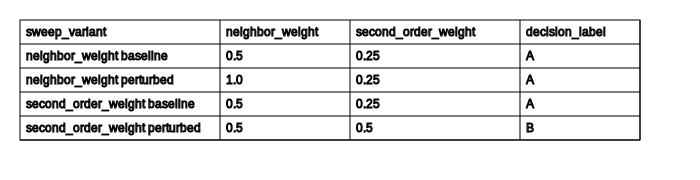
\includegraphics[width=\linewidth]{figures/figure2_primary_sweep.pdf}
  \caption{Primary representational sweep. Each column corresponds to a representation variant defined by its weight parameter setting. Decision identity (A or B) is assigned by the equivalence policy based on the route node sequence. The neighbor weight sweep (left) shows identity persistence; the second-order weight sweep (right) shows a boundary.}
  \label{fig:primary-sweep}
\end{figure}

\begin{figure}[t]
  \centering
  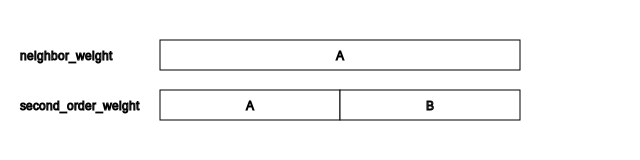
\includegraphics[width=\linewidth]{figures/figure3_identity_persistence.pdf}
  \caption{Identity persistence regions derived from the sweep in Figure~\ref{fig:primary-sweep}. The neighbor weight parameter spans a single persistence region (Decision~A). The second-order weight parameter spans two regions (A and B) separated by a boundary between 0.25 and 0.5.}
  \label{fig:persistence}
\end{figure}

\begin{figure}[t]
  \centering
  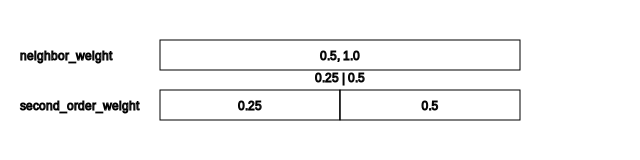
\includegraphics[width=\linewidth]{figures/figure4_boundary_fracture.pdf}
  \caption{Boundary and fracture localization. The neighbor weight sweep shows no boundary (\texttt{route\_changed = false}). The second-order weight sweep shows a boundary between 0.25 and 0.5 (\texttt{route\_changed = true}, \texttt{edge\_order\_changed = true}).}
  \label{fig:boundary}
\end{figure}

Table~\ref{tab:sweep-summary} summarizes the sweep results.

\begin{table}[t]
\centering
\caption{Summary of representational sweep results.}
\label{tab:sweep-summary}
\smallskip
\tablestyle
\rowcolors{2}{tableShade}{white}
\begin{tabular}{@{\hskip 8pt}l l c c l@{\hskip 8pt}}
\toprule
\rowcolor{white}
\textbf{Sweep parameter} & \textbf{Value} & \textbf{Decision} & \textbf{Nodes} & \textbf{Boundary?} \\
\midrule
\texttt{neighbor\_weight} & 0.5 & A & 16 & \\
\texttt{neighbor\_weight} & 1.0 & A & 16 & No \\
\texttt{second\_order\_weight} & 0.25 & A & 16 & \\
\texttt{second\_order\_weight} & 0.5 & B & 14 & Yes \\
\bottomrule
\end{tabular}
\end{table}

\subsection{Replay Verification}

We verify replay determinism for a decision produced by the sweep. The replay procedure loads the stored raw output from its persisted URI, recomputes the equivalence policy identifier, extracts the decision payload, and recomputes both the payload hash and the decision identifier.

All recomputed values match the persisted values exactly (Table~\ref{tab:replay}, Figure~\ref{fig:replay}):

\begin{table}[ht]
\centering
\caption{Replay verification results for decision \texttt{dec\_e280\ldots}.}
\label{tab:replay}
\smallskip
\tablestyle
\rowcolors{2}{tableShade}{white}
\begin{tabular}{@{\hskip 8pt}l l l@{\hskip 8pt}}
\toprule
\rowcolor{white}
\textbf{Field} & \textbf{Persisted} & \textbf{Recomputed} \\
\midrule
Policy ID & \texttt{pol\_d8da3e00e9584eb1} & \texttt{pol\_d8da3e00e9584eb1} \\
Payload hash & \texttt{3a9d63ac28378116} & \texttt{3a9d63ac28378116} \\
Decision ID & \texttt{dec\_e28092c4dc33b8f1} & \texttt{dec\_e28092c4dc33b8f1} \\
\bottomrule
\end{tabular}
\end{table}

The replay writes no new rows and modifies no database state. Table counts before and after replay are identical (1 engine run, 1 decision, 1 f\_map entry). This confirms that the content-addressing chain from raw output through policy application to decision identity is deterministic and end-to-end auditable.

\begin{figure}[t]
  \centering
  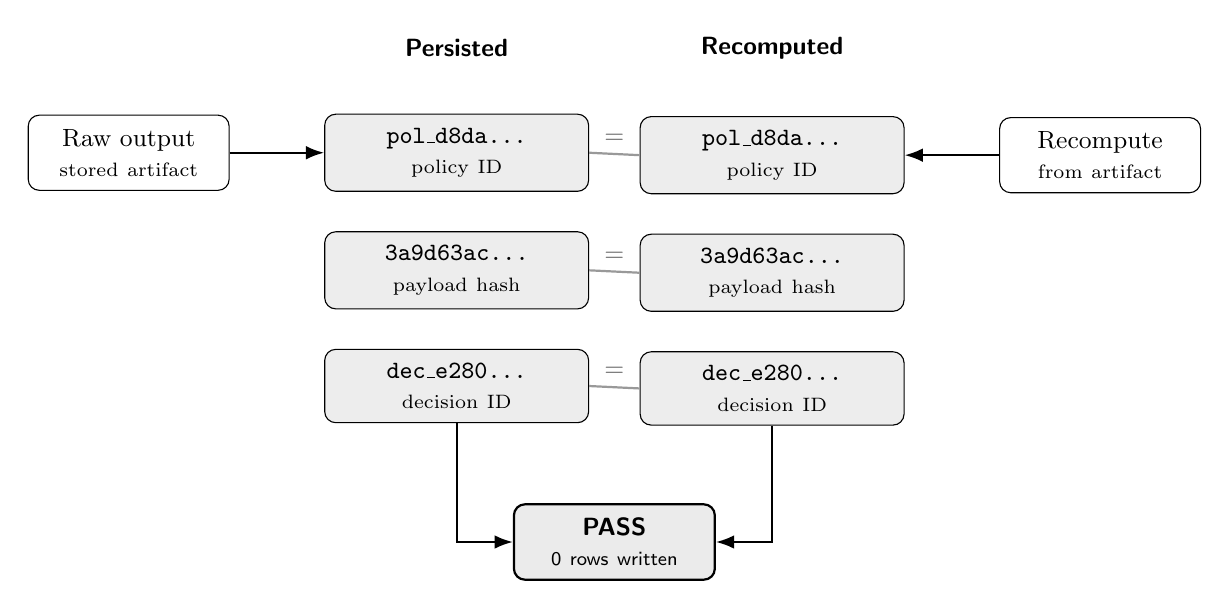
\begin{tikzpicture}[
    node distance=5mm and 8mm,
    box/.style={draw, rounded corners, align=center, inner sep=5pt, text width=30mm, font=\small},
    artifact/.style={box, fill=tableShade},
    result/.style={box, fill=black!8, font=\small\sffamily},
    arrow/.style={-Latex, thick},
    eq/.style={font=\small\sffamily, text=black!60}
  ]
  % Left column: persisted
  \node[font=\small\bfseries\sffamily] (plabel) {Persisted};
  \node[artifact, below=6mm of plabel] (ppol) {\texttt{pol\_d8da\ldots}\\{\scriptsize policy ID}};
  \node[artifact, below=of ppol] (phash) {\texttt{3a9d63ac\ldots}\\{\scriptsize payload hash}};
  \node[artifact, below=of phash] (pdec) {\texttt{dec\_e280\ldots}\\{\scriptsize decision ID}};

  % Right column: recomputed
  \node[font=\small\bfseries\sffamily, right=22mm of plabel] (rlabel) {Recomputed};
  \node[artifact, below=6mm of rlabel] (rpol) {\texttt{pol\_d8da\ldots}\\{\scriptsize policy ID}};
  \node[artifact, below=of rpol] (rhash) {\texttt{3a9d63ac\ldots}\\{\scriptsize payload hash}};
  \node[artifact, below=of rhash] (rdec) {\texttt{dec\_e280\ldots}\\{\scriptsize decision ID}};

  % Equality checks
  \draw[thick, black!40] (ppol.east) -- node[eq, above] {$=$} (rpol.west);
  \draw[thick, black!40] (phash.east) -- node[eq, above] {$=$} (rhash.west);
  \draw[thick, black!40] (pdec.east) -- node[eq, above] {$=$} (rdec.west);

  % Source arrow
  \node[box, left=12mm of ppol, text width=22mm] (raw) {Raw output\\{\scriptsize stored artifact}};
  \draw[arrow] (raw.east) -- (ppol.west);

  % Recompute arrow
  \node[box, right=12mm of rpol, text width=22mm] (engine) {Recompute\\{\scriptsize from artifact}};
  \draw[arrow] (engine.west) -- (rpol.east);

  % Verdict
  \node[result, below=10mm of $(pdec.south)!0.5!(rdec.south)$, text width=22mm, line width=0.8pt] (verdict) {\textbf{PASS}\\{\scriptsize 0 rows written}};
  \draw[arrow] (pdec.south) |- (verdict.west);
  \draw[arrow] (rdec.south) |- (verdict.east);

  \end{tikzpicture}
  \caption{Replay verification. Persisted identifiers (left) are compared against values recomputed from stored artifacts (right). All three fields match exactly. No rows are written and no database state is modified.}
  \label{fig:replay}
\end{figure}


\section{Related Work}

The sensitivity of analytical conclusions to representational and analytic choices has been documented across multiple disciplines. This section situates the decision-valued mapping framework relative to existing work on analytic flexibility, reproducibility infrastructure and provenance systems. Table~\ref{tab:comparison} summarizes the key distinctions.

\subsection{Analytic Flexibility and Multiverse Methods}

The dependence of statistical conclusions on analytic choices has been examined through several complementary lenses. Specification curve analysis~\cite{simonsohn2020specification} evaluates how reported effects vary across defensible analytic specifications. Multiverse analysis~\cite{steegen2016increasing} extends this by jointly varying data processing and model specification decisions to characterize the full space of results consistent with a dataset. The same instability appears even when researchers follow pre-registered protocols, through implicit degrees of freedom that shape findings absent deliberate p-hacking~\cite{gelman2013garden}. The scale of this effect in observational studies is substantial, with effect estimates fluctuating across model specifications~\cite{patel2015assessment}.

Decision-valued mapping shares the premise that analytic conclusions depend on choices that are often left implicit. Specification curve and multiverse analyses operate on continuous effect estimates such as regression coefficients and p-values, then visualize their distribution. Decision-valued maps operate on discrete outcome identities and characterize the topology of representation space, identifying which regions preserve identity and where boundaries form, producing a partition rather than a distribution.

\subsection{Sensitivity Analysis}

Sensitivity analysis quantifies how variation in model inputs contributes to variation in model outputs, typically through variance decomposition or derivative-based indices over continuous output spaces~\cite{saltelli2008global}. Decision-valued mapping differs in that it does not decompose output variance or compute sensitivity indices. Instead, it directly observes whether a discrete outcome changes or persists under representation variation. Decision-valued mapping is compatible with sensitivity analysis, since sensitivity indices could be computed over a binarized decision map, but it does not require or assume a continuous output metric.

\subsection{Reproducibility in Machine Learning}

Pipelines satisfying identical training criteria can yield predictors with divergent behavior under distribution shift~\cite{damour2022underspecification}. Deep reinforcement learning results are sensitive to implementation details and hyperparameter choices in ways that standard reporting obscures~\cite{henderson2018deep}, and variance accounting across machine learning benchmarks has been formalized to quantify this effect~\cite{bouthillier2021accounting}. Reproducibility checklists~\cite{pineau2021improving} encourage reporting of experimental details but do not enforce content-addressed provenance or deterministic replay.

Decision-valued mapping addresses a related but distinct problem. Rather than documenting variability in performance metrics across training runs or hyperparameter settings, it isolates representational variation as an independent variable and tracks its effect on discrete outcome identity under fixed snapshots and engines. Decision-valued mapping complements reproducibility checklists by providing a lower-level infrastructure for testing whether specific outcomes are stable under specific representational changes.

\subsection{Provenance and Workflow Systems}

General-purpose provenance vocabularies record the derivation history of computational artifacts~\cite{moreau2013prov}. Workflow provenance for scientific computations~\cite{freire2012provenance}, experiment tracking for machine learning pipelines~\cite{zaharia2018accelerating}, standardized workflow definitions for reproducible execution~\cite{amstutz2016common} and lineage tracking for fault-tolerant distributed computation~\cite{zaharia2012resilient} all address aspects of this problem.

DecisionDB is narrower than these systems in scope and more specific in its invariants. Rather than managing arbitrary workflows or tracking general-purpose provenance graphs, it enforces a specific structure with immutable snapshots, declared representation families, fixed engines and equivalence policies that reduce raw output to discrete identities. The content-addressing scheme ensures that identical inputs always produce identical identifiers; replay verification checks end-to-end consistency of the provenance chain. This specificity enables the decision-valued map as a queryable diagnostic object, which general-purpose provenance systems do not directly support.

\begin{table}[t]
\centering
\caption{Summary comparison between decision-valued mapping and related approaches.}
\label{tab:comparison}
\smallskip
\tablestyle
\rowcolors{2}{tableShade}{white}
\begin{tabular}{@{\hskip 6pt}R{30mm} R{40mm} R{44mm}@{\hskip 6pt}}
\toprule
\rowcolor{white}
Dimension & Typical approaches & Decision-valued mapping \\
\midrule
Object of analysis & Continuous effect estimates, variance, p-values & Discrete decision identities \\
Variation source & Model specs, preprocessing, hyperparameters & Representation parameters under fixed snapshot and engine \\
Output characterization & Distributions, sensitivity indices, specification curves & Persistence regions, boundaries, fractures \\
Infrastructure & Logging, provenance metadata, workflow graphs & Content-addressed, replayable decision maps \\
\bottomrule
\end{tabular}
\end{table}

\subsection{Infrastructural Precedents}

The approach follows a pattern observed in the development of foundational abstractions. Abstract data types~\cite{liskov1974programming} separated representation from observable behavior, enabling systems to evolve internally without collapsing external guarantees. Write-ahead logging~\cite{gray1993transaction} transformed durability from an ad-hoc property into an auditable, replayable state transition protocol. In both cases, the contribution was not a novel computational procedure but a diagnostic layer that made structural dependence explicit and testable.

Each decision occurs within an arena defined by a snapshot, an engine and a query. The protocol records how outcome identity evolves across representational variants within that arena. Methods that adapt model parameters during evaluation concentrate effort on producing stronger solutions within that arena. The present protocol instead addresses reuse, asking whether the recorded context is sufficient to justify carrying a discrete outcome across representations and downstream consumers. Decision-valued mapping extends this lineage to analytical pipelines whose outputs are discrete, consequential and contingent on representational choice.


\section{Limitations}

\textbf{Discrete outcomes only.} The framework applies to systems whose outputs can be reduced to discrete identities via a declared equivalence policy. Continuous outputs (e.g., probability distributions, regression surfaces) are out of scope unless such a reduction is explicitly defined. The choice of equivalence policy directly determines what counts as ``the same outcome,'' and different policies applied to the same raw output will in general produce different decision maps.

\textbf{Fixed snapshot and engine.} All results assume a frozen snapshot and a fixed engine. Any change to the input data, model parameters, or execution logic constitutes a new analytical context. The framework does not track how decision maps evolve across snapshot or engine versions; each combination requires a separate analysis.

\textbf{Empirical coverage.} The reported sweeps cover two representation parameters (\texttt{neighbor\_weight} at values 0.5 and 1.0; \texttt{second\_order\_weight} at values 0.25 and 0.5) applied to a single graph snapshot with a single origin-destination pair. The representation space is sampled at four points total. Unobserved regions of representation space remain unconstrained: persistence regions and boundaries identified here may not generalize to finer parameter grids, different origin-destination pairs, or different graph topologies.

\textbf{Single domain.} The empirical demonstration uses graph routing. The framework is designed to be domain-agnostic, but we have not validated it on classification, resource allocation, or other pipeline types. Applying the framework to a new domain requires defining an appropriate equivalence policy, which involves domain-specific judgment about what constitutes ``the same outcome.''

\textbf{No causal claims.} Observing that a boundary exists between two parameter values does not explain why it exists. The framework is diagnostic, not explanatory. It identifies where decision identity changes but does not attribute the change to any specific mechanism within the engine or the representation construction.

\textbf{Scalability.} The current implementation uses SQLite and has been tested with single-digit representation families. Scaling to large parameter grids (hundreds or thousands of representations) would require evaluation of storage, query performance, and sweep orchestration, which we have not performed.


\section{Conclusion}

This paper introduced decision-valued maps as a diagnostic object for characterizing how discrete outcomes depend on representational choices. The object is a mapping from representations to decision identities, evaluated under a fixed snapshot and engine, and materialized through content-addressed identifiers and immutable artifacts.

DecisionDB implements this framework through a five-stage sweep protocol, a five-table relational schema, and a replay verification procedure. In a graph routing demonstration, one representation parameter preserves route identity across its tested range while another induces a discrete route change. Replay verification confirmed that all persisted decision identifiers are deterministically recoverable.

The framework is limited by its restriction to discrete outcomes, its reliance on fixed snapshots and engines, and the narrow empirical coverage reported here. Extending the approach to finer parameter grids, additional domains, and cross-snapshot comparison are directions for future work.

The contribution is infrastructural. Making representational dependence observable does not improve outcomes, but it is a prerequisite for understanding when discrete outcomes can be trusted and when they cannot.


\bibliographystyle{plainnat}
\bibliography{bibliography}

\end{document}
